\documentclass[10pt]{article}
\usepackage[letterpaper,margin=0.60in]{geometry}
\usepackage[T1]{fontenc}
\usepackage{lmodern}
\usepackage{microtype}
\usepackage{amsmath,amssymb,amsthm,mathtools}
\usepackage{xcolor}
\usepackage{titlesec}
\usepackage[most]{tcolorbox}
\usepackage{graphicx,booktabs}
\usepackage[font=small,labelfont=bf,skip=5pt]{caption}
\usepackage{hyperref}

\definecolor{ink}{HTML}{000000}
\definecolor{accent}{HTML}{000000}
\definecolor{boxfill}{HTML}{F4F7F9}
\definecolor{boxline}{HTML}{CBD9E3}
\hypersetup{colorlinks=true,linkcolor=accent,urlcolor=accent,citecolor=accent,
  pdftitle={Finite Observation and Broader Physical Processes},pdfauthor={J. R. Landers}}
\color{ink}
\titleformat{\section}{\large\bfseries\color{accent}}{}{0pt}{}
\titlespacing*{\section}{0pt}{0.75em}{0.25em}
\setlength{\parindent}{0pt}
\setlength{\parskip}{0.40em}
\newtcolorbox{resultbox}{enhanced,breakable,colback=boxfill,colframe=boxline,
  boxrule=0.45pt,arc=3.5mm,left=7.5pt,right=7.5pt,top=5pt,bottom=5pt,
  before skip=0.45em,after skip=0.45em}
\newtcolorbox{highlightbox}{enhanced,breakable,colback=boxfill,colframe=boxline,
  boxrule=0.45pt,arc=3.5mm,left=7.5pt,right=7.5pt,top=7pt,bottom=7pt,
  before skip=9.5pt,after skip=8pt}
\newcounter{claim}
\newcommand{\claim}[2]{\refstepcounter{claim}\label{#1}\textbf{#2 \theclaim.}}
\newcommand{\TV}{\operatorname{TV}}
\newcommand{\KL}{D_{\mathrm{KL}}}
\newcommand{\Law}{\mathcal L}
\newcommand{\R}{\mathbb R}
\newcommand{\eps}{\varepsilon}
\newcommand{\obs}{\mathcal O}
\newcommand{\norm}[1]{\left\lVert#1\right\rVert}
\title{\vspace{-2.3em}\textbf{Finite Observation and Broader Physical Processes}}
\author{J. R. Landers}
\date{}

\begin{document}
\maketitle
\vspace{-1.35em}
\small
\begin{abstract}
A system can pass every test of a simple model over a finite experiment and
still belong to larger dynamics that dominate it later. This note makes that
statement quantitative. We first bound how well noisy, adaptive measurements
can tell two models apart, then build an explicit pair: two coupled Hamiltonian
oscillators whose visible coordinate tracks a single isolated oscillator as
closely as one likes over a chosen window, yet differs from it by a full
amplitude afterwards. The total energy stays bounded, and letting the observer
actively drive the system on a finite impulse budget does not break the bound.
If the observer records only the sign of position, the two models agree
\emph{exactly} until the slow envelope first vanishes. A separate Poisson
model---an assumption, not a consequence of the construction---says precisely
when further relevant scales exist almost surely. Every bound is proved.
\end{abstract}

\section*{The gap between fitting a record and knowing a system}
Suppose you watch a system for a while and a simple model fits: residuals sit
at the noise level and predictions hold up. What does that license? It licenses
prediction over the range you tested. It does not by itself rule out that the
system is one part of larger dynamics whose remaining parts are quiet during
your record and loud afterwards. This note measures the gap between the two
claims.

\begin{highlightbox}
\centering
\textbf{A model can fit a finite record arbitrarily well and still omit
dynamics that dominate the system later.}
\end{highlightbox}

\emph{Fit arbitrarily well} has a precise meaning here: no protocol in a
stated class---fixed noise level, fixed number of readings, adaptive sampling,
bounded driving---distinguishes the two models better than chance by more than
$\eps$. \emph{Larger} means having a characteristic timescale longer than the
record; the hidden dynamics need not sit anywhere else in space. In our example
everything happens inside a two-degree-of-freedom mechanical system that
exchanges energy slowly.

The argument runs in five steps. A geometric estimate asks how much of a slow
variation fits inside a short window. A statistical bound turns small signal
differences into a limit on detection. The oscillator pair then supplies a
difference that is invisible early and total later, and a second bound shows
that active probing on a finite budget does not help. A coarse-graining hides
the difference exactly rather than approximately. A final, separate section
asks a different question: how likely is a further scale in the first place?

The tools are standard graduate material---Taylor remainders, Gaussian
likelihood ratios, normal modes, Poisson point processes---and what they buy is
a clean separation between predictive reliability and physical completeness.
Noise is essential to the story: with noiseless data, spectral methods can
resolve arbitrarily close frequencies from a single snapshot~\cite{liao}.

\section*{What fits inside an observation window}
Begin with the simplest version of the question, one with no dynamics in it at
all. The observer has access to a closed ball $B_R(x_0)\subset\R^d$ carrying a
Euclidean metric, and measures a scalar observable $f$, differentiable near
that ball. The radius $R$ is the reach of the record---how far the measurements
extend---not the size or lifetime of the observer. If the ball mixes spatial and
temporal coordinates, they must first be put into common units by an explicit
physical normalization.

Fix an amplitude scale $A>0$ and a variation scale $L>0$, and suppose
$\norm{\nabla f}\leq A/L$ on the ball. This inequality does all the work below,
and we assume it rather than derive it: saying that a process has scale $L$
does not by itself imply it.

\begin{resultbox}
\claim{prop:geometry}{Proposition} \textbf{Local variation and curvature.}
If $\norm{\nabla f(x)}\leq A/L$ throughout $B_R(x_0)$, then
\begin{equation}
\sup_{x\in B_R(x_0)}|f(x)-f(x_0)|\leq A\frac RL.
\label{eq:gradient}
\end{equation}
If instead $f$ is twice continuously differentiable and
$\norm{\nabla^2 f(x)}_{\mathrm{op}}\leq A/L^2$, then its affine approximation
$\ell(x)=f(x_0)+\nabla f(x_0)\cdot(x-x_0)$ obeys
\begin{equation}
\sup_{x\in B_R(x_0)}|f(x)-\ell(x)|\leq\frac A2\left(\frac RL\right)^2.
\label{eq:curvature}
\end{equation}
\end{resultbox}
\begin{proof}
Write $h=x-x_0$ and $\gamma(u)=x_0+uh$, $0\leq u\leq1$. The segment stays
inside the ball. The fundamental theorem of calculus gives
\[
f(x)-f(x_0)=\int_0^1\nabla f(\gamma(u))\cdot h\,du,
\]
whose absolute value is at most $A\norm h/L\leq AR/L$.
For the second statement, applying the same theorem twice gives the integral
remainder
\[
f(x)-\ell(x)=\int_0^1(1-u)h^{\mathsf T}\nabla^2 f(\gamma(u))h\,du.
\]
Its absolute value is at most
$(A/L^2)\norm h^2\int_0^1(1-u)\,du\leq AR^2/(2L^2)$.
\end{proof}

Read the two bounds as statements about what a record can look like. When
$R\ll L$, the first says the observable is constant to within $AR/L$: a slow
process is indistinguishable from a fixed value. The second says that even
after fitting value and slope, the leftover curvature is only $A(R/L)^2/2$, so
the process looks like a simple trend. Neither bound claims the dynamics are
hidden in principle---a different observable of the same system may show the
variation at once.

\section*{From a small signal difference to a limit on detection}
A difference of size $b$ between two signals is not yet a difference an
experiment can detect. That depends on the noise, on how many readings are
taken, and on what the observer may do between them. We fix all of this in a
protocol $\obs$: the accessible coordinates, the observation window, the
measurement noise, the sampling policy (which may be adaptive), and any forcing
permitted. Each physical model then induces a law $P^{\obs}$ on the complete
record---every reading, in order, together with the actions taken. Define
\[
\TV(P,Q)=\sup_B|P(B)-Q(B)|,
\qquad
\KL(P\Vert Q)=\int\log\!\left(\frac{dP}{dQ}\right)dP,
\]
where relative entropy uses natural logarithms and is infinite when absolute
continuity fails. Equal record laws mean the protocol cannot distinguish the
models at all; we call two laws \emph{$\eps$-unresolved} when their total
variation is at most $\eps$. This approximate relation need not be transitive,
so $\eps$-unresolvedness should not be chained.

\begin{resultbox}
\claim{lem:observation}{Lemma} \textbf{A bound for adaptive Gaussian records.}
Consider two models with at most $n$ scalar readings. Given the same preceding
record, reading $i$ has respective conditional means $m_{0,i},m_{1,i}$ and
common variance $\sigma^2>0$. Assume
$|m_{1,i}-m_{0,i}|\leq b$ for every allowed preceding record and action.
Policies use only preceding readings and independent randomization. Then
\begin{equation}
\KL(P_1^{\obs}\Vert P_0^{\obs})\leq\frac{nb^2}{2\sigma^2},
\qquad
\TV(P_1^{\obs},P_0^{\obs})\leq
\min\!\left\{1,\frac{\sqrt n\,b}{2\sigma}\right\}.
\label{eq:record-bound}
\end{equation}
At equal prior probabilities, the minimum classification error is
\begin{equation}
e_* = \frac{1-\TV(P_1^{\obs},P_0^{\obs})}{2}.
\label{eq:testing}
\end{equation}
\end{resultbox}
\begin{proof}
For Gaussian densities of common variance, taking the expectation of their
log-density ratio gives $(m_1-m_0)^2/(2\sigma^2)$. Factor the joint record
density into successive conditional densities. The expected log of their
product is the sum of the expected conditional log-density ratios, so
\[
\KL(P_1^{\obs}\Vert P_0^{\obs})
=\sum_{i=1}^n\mathbb E_1
 \frac{(m_{1,i}-m_{0,i})^2}{2\sigma^2}
\leq\frac{nb^2}{2\sigma^2}.
\]
Conditional on the same history, the policy chooses the same action law in
both models; it contributes no additional likelihood ratio. Independent
randomization can be included in the record. An early stopping rule is handled
by appending model-independent dummy readings after stopping.

For completeness, the variation--entropy inequality used here follows by
coarse-graining to an event $B$. Write $p=P(B)$ and $q=Q(B)$. Jensen's
inequality for the density ratio separately on $B$ and $B^c$ gives
\[
\KL(P\Vert Q)\geq
p\log(p/q)+(1-p)\log((1-p)/(1-q))=:d(p,q).
\]
For $0<p,q<1$, as a function of $p$, $d(q,q)=\partial_p d(q,q)=0$ and
$\partial_p^2d(p,q)=1/[p(1-p)]\geq4$. Integrating twice yields
$d(p,q)\geq2(p-q)^2$; boundary cases follow by limits. Taking the supremum
over $B$ proves $\TV(P,Q)\leq\sqrt{\KL(P\Vert Q)/2}$.
Finally, a test choosing model 1 on $B$ has error
$[P_0(B)+P_1(B^c)]/2=[1-(P_1(B)-P_0(B))]/2$.
Optimizing over $B$, or the corresponding likelihood-ratio test, gives
\eqref{eq:testing}; randomized tests cannot improve the optimum.
\end{proof}

The content of the lemma is that adaptivity does not help. A clever sampling
policy can choose when and where to look, but given the same past record it
chooses the same way under either model, so the choice contributes nothing to
the likelihood ratio. The observer is left with $n$ readings, each worth at most
$b^2/2\sigma^2$ nats.

Combining Proposition~\ref{prop:geometry} and Lemma~\ref{lem:observation},
adaptive samples of $f$ and its constant approximation in $B_R(x_0)$ satisfy
\begin{equation}
\TV(P_f^{\obs},P_{f(x_0)}^{\obs})
\leq\min\!\left\{1,\frac{\sqrt n A}{2\sigma}\frac RL\right\}.
\label{eq:scale-observation}
\end{equation}
So $L\geq\sqrt n AR/(2\sigma\eps)$ suffices for $\eps$-unresolvedness against
the constant model, and comparing against the affine approximation instead
replaces the bound by $\sqrt n A(R/L)^2/(4\sigma)$. One caveat on the
comparison: the approximating value and slope are fixed model parameters, not
quantities fitted to the same data. A composite null estimated from the record
needs its own treatment.

\section*{A hidden degree of freedom that matters later}
Indistinguishability on its own is not interesting: two models can be
indistinguishable because they barely differ. What we want is a pair that no
early experiment separates and whose later behaviour differs completely, with no
runaway energy making the difference cheap. Two coupled oscillators do it. All
masses are one, and the reference model is a single visible coordinate $q$ with
momentum $p$ and Hamiltonian
\begin{equation}
H_0(q,p)=\tfrac12p^2+\tfrac12\omega^2q^2,
\qquad \omega>0.
\label{eq:H0}
\end{equation}
The extension adds a coordinate $Q$ and momentum $P$:
\begin{equation}
H_\delta(q,p,Q,P)
=\tfrac12(p^2+P^2)+\tfrac12(\omega^2+\delta^2)(q^2+Q^2)
 +2\omega\delta qQ,
\qquad 0<\delta\leq\omega/2.
\label{eq:H1}
\end{equation}
The observer measures $q$ and, when allowed, drives it; $Q$, $P$, and the
spring parameters are inaccessible. Note that the extension changes two things
at once: it adds the coordinate $Q$, and it shifts the local stiffness from
$\omega^2$ to $\omega^2+\delta^2$. Both are part of what is being proposed.

\begin{resultbox}
\claim{prop:modes}{Proposition} \textbf{Stable dynamics and delayed modulation.}
For initial data $q(0)=A>0$, $p(0)=0$, and $Q(0)=P(0)=0$ in the extension,
\begin{equation}
q_0(t)=A\cos(\omega t),\qquad
q_\delta(t)=A\cos(\omega t)\cos(\delta t),\qquad
Q_\delta(t)=-A\sin(\omega t)\sin(\delta t).
\label{eq:solutions}
\end{equation}
The extended Hamiltonian is positive definite, and its conserved energy is
\begin{equation}
E_\delta=\tfrac12A^2(\omega^2+\delta^2)
\leq\tfrac58 A^2\omega^2.
\label{eq:energy}
\end{equation}
\end{resultbox}
\begin{proof}
The orthogonal canonical transformation
$u=(q+Q)/\sqrt2$, $v=(q-Q)/\sqrt2$, with momenta
$p_u=(p+P)/\sqrt2$, $p_v=(p-P)/\sqrt2$, gives
\[
H_\delta=\tfrac12[p_u^2+(\omega+\delta)^2u^2]
          +\tfrac12[p_v^2+(\omega-\delta)^2v^2].
\]
Both frequencies are positive, proving positive definiteness and stability.
The initial normal coordinates are $u(0)=v(0)=A/\sqrt2$ with zero momenta.
Their cosine solutions, transformed back and simplified by the sum and
difference identities, give \eqref{eq:solutions}. Evaluating the autonomous
Hamiltonian at the initial state gives \eqref{eq:energy}.
\end{proof}

The transformation in the proof diagonalizes the extension into two
independent oscillators at frequencies $\omega\pm\delta$, and everything follows
from that. Both frequencies are real and positive, so the motion is bounded and
the energy conserved. Projected back onto the visible coordinate, the two nearby
frequencies beat: a carrier at $\omega$ underneath an envelope at $\delta$. The
hidden process is slow rather than large---timescale $1/\delta$---and it merely
moves a fixed amount of energy back and forth.

\begin{resultbox}
\claim{thm:passive}{Theorem} \textbf{Early ambiguity and a later full-amplitude difference.}
For at most $n$ adaptive position readings on $[0,T]$ with independent Gaussian
noise of standard deviation $\sigma>0$ and no forcing,
\begin{equation}
\TV(P_\delta^{\obs},P_0^{\obs})
\leq\min\!\left\{1,\frac{\sqrt n A\delta^2T^2}{4\sigma}\right\}.
\label{eq:passive}
\end{equation}
For any positive integer $m$, choose
\begin{equation}
\delta=\frac{\omega}{4m},\qquad
T_* = \frac{\pi}{2\delta}=\frac{2\pi m}{\omega}.
\label{eq:late-time}
\end{equation}
Then $q_0(T_*)=A$ and $q_\delta(T_*)=0$. For fixed
$A,\omega,T,n,\sigma$, the bound in \eqref{eq:passive} tends to zero as
$m\to\infty$, while this later discrepancy remains exactly $A$.
\end{resultbox}
\begin{proof}
From \eqref{eq:solutions} and $0\leq1-\cos z\leq z^2/2$,
\[
|q_\delta(t)-q_0(t)|
\leq A[1-\cos(\delta t)]\leq A\delta^2T^2/2
\quad(0\leq t\leq T).
\]
Apply Lemma~\ref{lem:observation} with $b=A\delta^2T^2/2$. At the selected
time, $\omega T_*=2\pi m$ and $\delta T_*=\pi/2$, proving the exact late
values. Finally $\delta^2=\omega^2/(16m^2)\to0$.
\end{proof}

This theorem is the core of the note, so read \eqref{eq:passive} and
\eqref{eq:late-time} together. Shrinking $\delta$ makes the early record
arbitrarily uninformative---the bound falls like $1/m^2$---while the eventual
discrepancy stays exactly $A$, one full amplitude, however small $\delta$ is.
Only the time at which it appears moves out, to $T_*=2\pi m/\omega$. There is no
tradeoff in which a well-hidden extension must also be a weak one.

Nor is the late effect a small correction riding on the visible motion. At
$T_*$ both positions are zero, but $p_\delta(T_*)=-A\delta$ while
$P_\delta(T_*)=-A\omega$: the hidden momentum carries the fraction
$\omega^2/(\omega^2+\delta^2)\to1$ of the total energy. A degree of freedom that
started with none of the energy ends up with essentially all of it.

\section*{Can active probing reveal the extension?}
An observer with a controllable system does more than watch it. Pushing on $q$
and seeing how it responds is exactly how one would look for an extra spring, so
we allow it. Let a locally integrable force $u(t)$ act on $q$ in both models,
subject to a pathwise budget
\begin{equation}
\int_0^T|u(t)|\,dt\leq J.
\label{eq:impulse}
\end{equation}
on total absolute impulse. The budget is what makes the question non-trivial:
an unbounded push separates any two models. Between readings the force may
depend on everything recorded so far plus independent randomization, sampling
times are nondecreasing and may be adaptive, and the same policy is applied to
both models. What the controller may not use is state it has not recorded.

\begin{resultbox}
\claim{thm:active}{Theorem} \textbf{A uniform bound under bounded probing.}
For every such policy with at most $n$ position readings of noise level $\sigma$,
\begin{equation}
\TV(P_\delta^{\obs},P_0^{\obs})
\leq\min\!\left\{1,
\frac{\sqrt n\,\delta^2}{2\sigma}
\left(\frac{AT^2}{2}+\frac{JT^3}{6}\right)\right\}.
\label{eq:active}
\end{equation}
During probing, each model's instantaneous mechanical energy satisfies
\begin{equation}
H(t)\leq\tfrac12\bigl(\sqrt{2H(0)}+J\bigr)^2.
\label{eq:forced-energy}
\end{equation}
\end{resultbox}
\begin{proof}
For a prescribed force history, linearity gives
$q_a^u(t)=q_a(t)+\int_0^tG_a(t-s)u(s)\,ds$, where $a=0,\delta$ and
\[
G_0(r)=\frac{\sin(\omega r)}{\omega},\qquad
G_\delta(r)=\frac12\left[
\frac{\sin((\omega+\delta)r)}{\omega+\delta}
+\frac{\sin((\omega-\delta)r)}{\omega-\delta}\right].
\]
To bound the difference, write $g_\nu(r)=\int_0^r\cos(\nu s)\,ds$.
Differentiating under the integral yields
$|\partial_\nu^2g_\nu(r)|
=|\int_0^r-s^2\cos(\nu s)\,ds|\leq r^3/3$.
Taylor's formula about $\nu=\omega$, averaged at $\omega\pm\delta$, cancels
the linear terms and gives
\[
|G_\delta(r)-G_0(r)|\leq\delta^2r^3/6.
\]
Consequently, for $t\leq T$ and every force satisfying \eqref{eq:impulse},
\begin{equation}
|q_\delta^u(t)-q_0^u(t)|
\leq\delta^2\left(\frac{AT^2}{2}+\frac{JT^3}{6}\right)=:b_J.
\label{eq:forced-discrepancy}
\end{equation}
In an adaptive experiment, fix a common preceding record and random seed.
The policy has then generated the same force history and next sampling time
under either model. Thus \eqref{eq:forced-discrepancy} bounds each conditional
mean difference, even though force histories on two separately realized runs
need not coincide. Lemma~\ref{lem:observation} proves \eqref{eq:active}.

For energy, Hamilton's equations with the external force give
$\dot H=pu$. Positive definiteness implies $|p|\leq\sqrt{2H}$.
For $a>0$, $d\sqrt{2H+a}/dt=pu/\sqrt{2H+a}\leq|u|$ almost everywhere.
Integrating, then taking $a\downarrow0$, proves \eqref{eq:forced-energy}.
\end{proof}

The forced bound \eqref{eq:active} carries the same $\delta^2$ prefactor as
the passive one, with the impulse budget contributing a term of order $JT^3$.
Driving the system helps, but only by a fixed factor; it cannot beat the
$\delta^2\to0$ scaling. Inequality \eqref{eq:forced-energy} confirms that the
observer is not smuggling in unlimited resources: on an impulse budget $J$ the
energy stays bounded whatever the force does.

\begin{resultbox}
\claim{cor:closure}{Corollary} \textbf{No uniform finite-budget certificate of closure.}
Fix $A,\omega,T,\sigma>0$, a finite $n$, $J\geq0$, and $0<\eps<1$.
There is a nonzero $\delta=\omega/(4m)$ such that \emph{every} allowed policy
has $\TV(P_\delta^{\obs},P_0^{\obs})\leq\eps$, yet the unforced models differ
by $A$ at a later time $T_*>T$. Their unforced energies and energies during
allowed probing are bounded uniformly in $m$.
\end{resultbox}
\begin{proof}
Choose an integer $m$ large enough that $2\pi m/\omega>T$ and
\[
\frac{\sqrt n\,\omega^2}{32\sigma m^2}
\left(\frac{AT^2}{2}+\frac{JT^3}{6}\right)\leq\eps.
\]
Theorem~\ref{thm:active} applies uniformly over all permitted policies.
Theorem~\ref{thm:passive} supplies the unforced late difference, and
\eqref{eq:energy}--\eqref{eq:forced-energy} supply the uniform energy bounds.
\end{proof}

Read the corollary narrowly. It says that no fixed budget---$n$, $\sigma$,
$T$, $J$---certifies the absence of extensions \emph{uniformly} over a family
containing arbitrarily weak nonzero coupling. It does not say that any given
extension is undetectable: fix $\delta$, and a longer window, a finer
instrument, another observable, or a harder push will find it. The
full-amplitude late difference is also a statement about the unforced
trajectories; after an intervention the models still differ, but we do not claim
they differ by exactly $A$.

For passive observation the same inequalities price the alternative strategy of
waiting. Requiring classification error at most $\alpha<1/2$,
\eqref{eq:testing} and \eqref{eq:passive} require
\begin{equation}
n\geq\frac{16\sigma^2(1-2\alpha)^2}{A^2\delta^4T^4}
=\frac{256\sigma^2(1-2\alpha)^2}{\pi^4A^2}
\left(\frac{T_*}{T}\right)^4.
\label{eq:sample-cost}
\end{equation}
The sample count grows as the fourth power of $T_*/T$: reaching a consequence
a hundred times further out than the record costs on the order of $10^8$ times
the samples. This is a lower bound rather than an achievability claim, but the
tradeoff it makes explicit is the practical one---at fixed amplitude and noise,
buying access to a much later consequence from an early record gets expensive
fast.

\section*{A coarse record that hides the change exactly}
The concealment so far is approximate: the records differ, just by too little to
resolve. Coarse-graining can make it exact. Suppose the observer keeps only the
sign of position:
\[
\Pi(q)=\begin{cases}+,&q\geq0,\\-,&q<0.\end{cases}
\]
This partition sends an entire half-line to a single symbol. The extension
changes the amplitude of the visible oscillation, and a change in positive
amplitude moves \emph{within} a cell rather than across its boundary---so it
leaves no trace at all in the symbolic record until the envelope itself changes
sign.

\begin{resultbox}
\claim{prop:sign}{Proposition} \textbf{Exact symbolic agreement before the envelope zero.}
For the unforced solutions, at every $0\leq t<\pi/(2\delta)$,
\begin{equation}
\Pi(q_\delta(t))=\Pi(q_0(t)).
\label{eq:sign}
\end{equation}
For the discrete choices in \eqref{eq:late-time}, at $2T_*$ one has
$q_0(2T_*)=A$ and $q_\delta(2T_*)=-A$, so the symbols differ.
\end{resultbox}
\begin{proof}
Before $\pi/(2\delta)$ the factor $\cos(\delta t)$ is strictly positive.
Multiplication by it preserves sign, including common zeros under the stated
convention. At $2T_*$, $\omega(2T_*)=4\pi m$ and
$\delta(2T_*)=\pi$, giving the asserted values.
\end{proof}

Two caveats. This is an idealized sign-only channel: an observer who instead
thresholds a noisy amplitude does not get identical record laws, because the
amplitude changes the probability of a sign error---for that case the earlier
statistical bound applies. And a symbolic record that looks regular is not
thereby Markov; the unresolved phase can still control the next transition.

The connection to finite-horizon coarse descriptions is precise. In the
continuous-computation framework~\cite{landers,geometry} one compares a decoded
symbolic path with a finite-state reference process over a stated epoch. The
next statement transfers any \emph{independently established} approximation
bound from one model to the other; it assumes nothing about lumpability of the
oscillator's sign partition.

\begin{resultbox}
\claim{prop:transfer}{Proposition} \textbf{Transfer of a finite-horizon predictive description.}
Let a common decoder, possibly randomized, map experimental records to symbolic
paths, with laws $S_0$ and $S_1$. If
$\TV(P_1^{\obs},P_0^{\obs})\leq\eps$ and a reference path law $M$ satisfies
$\TV(S_0,M)\leq e$, then
\begin{equation}
\TV(S_1,M)\leq\min\{1,e+\eps\}.
\label{eq:transfer}
\end{equation}
\end{resultbox}
\begin{proof}
Let $K(B\mid r)\in[0,1]$ be the decoder's probability of a symbolic event $B$
given record $r$. Then
$S_1(B)-S_0(B)=\int K(B\mid r)\,d(P_1^{\obs}-P_0^{\obs})(r)$.
For any measurable $h\in[0,1]$, write
$h(r)=\int_0^1\mathbf1\{h(r)>s\}\,ds$; integration shows
$|\int h\,d(P_1^{\obs}-P_0^{\obs})|\leq\TV(P_1^{\obs},P_0^{\obs})$.
Hence $\TV(S_1,S_0)\leq\eps$. The triangle inequality gives the result.
\end{proof}

A model that is wrong about the physics can therefore inherit a certified
finite-horizon predictive description from the correct one, paying only $\eps$
in extra error. The certificate covers the stated preparation and record class,
not worst-case behaviour over all hidden states, and the horizon a given error
budget certifies is a lower bound on how long the description works, not the
point where it fails.

\section*{A worked example with numbers}
Take $A=\omega=1$, $\delta=1/400$, $T=10$, $n=100$, and $\sigma=0.1$, so that
$m=100$ and $T_*=200\pi\approx628.319$. The analytic bounds give
\[
\sup_{0\leq t\leq10}|q_\delta(t)-q_0(t)|\leq0.0003125,
\qquad \TV\leq0.015625,
\qquad e_*\geq0.4921875.
\]
The best possible equal-prior classifier therefore succeeds at most
$50.78125\%$ of the time on this protocol class---barely better than a coin
flip. Yet at $T_*$ the two models' position predictions differ by exactly one
full amplitude, and by $2T_*$ even their signs disagree.

\begin{figure}[htbp]
\centering
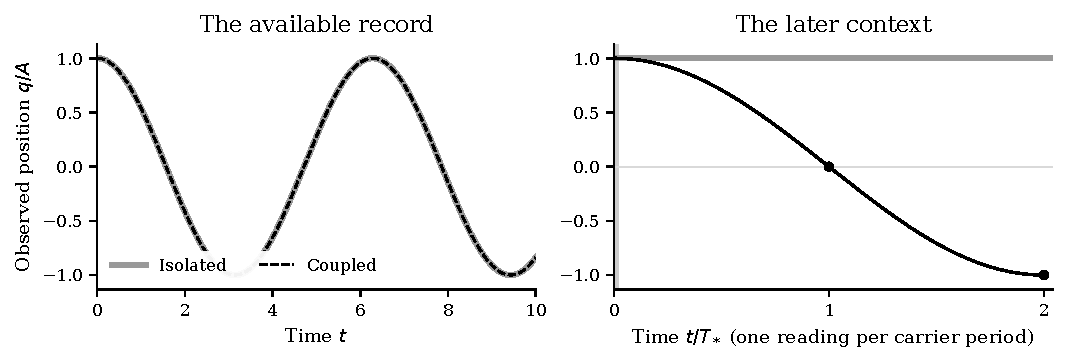
\includegraphics[width=0.95\linewidth]{finite_observation_figure.pdf}
\caption{One record, two physical explanations. Left: over the initial window,
the isolated and coupled positions nearly coincide. Right: sampling once per
carrier period makes the slow envelope visible; the isolated prediction remains
one while the coupled prediction eventually reaches zero and then minus one.
The narrow shaded interval marks the initial window. All plotted values are
exact solutions; connecting lines on the right guide the eye between samples.}
\label{fig:example}
\end{figure}

An independent integration of Hamilton's equations with relative tolerance
$10^{-10}$ and absolute tolerance $10^{-12}$ agreed with the exact visible
trajectory to within $3\times10^{-9}$ on $[0,T_*]$, with absolute energy drift
below $8\times10^{-9}$. For the test force $u(t)=0.1\sin(0.7t)$ on $[0,10]$,
the absolute impulse is at most $J=1$. The maximum computed position difference
was $0.00024649$, below the uniform bound $b_J=0.00135417$.
The forced record bound is then $\TV\leq0.067709$ for the same $n,\sigma$.
These runs check the implementation only; the inequalities above are proved
and do not rest on a fit to simulation.

\section*{How likely is a further scale in the first place?}
The oscillator construction shows that consequential hidden extensions exist. It
says nothing about how often they occur, and for that one needs a population
model---an assumption rather than a result. Read this section as the price of the
stronger claim: here is exactly what must be assumed for further relevant scales
to be certain.

Index processes by a characteristic scale $L\geq L_{\min}>0$. If scale
corresponds to a $d$-dimensional volume $V(L)=v_dL^d$, then
\[
\frac{dV}{V}=d\,\frac{dL}{L}.
\]
so equal multiplicative steps in scale are equal steps of log volume. This is a
choice of coordinate; it asserts nothing about where processes actually sit.

Assume the scales of relevant processes form a Poisson point process with
locally finite intensity measure
\begin{equation}
d\mu(L)=\eta(L)\frac{dV}{V}
=d\,\eta(L)\frac{dL}{L},\qquad \eta(L)\geq0.
\label{eq:intensity}
\end{equation}
Relevance here is stipulated, and the stipulation does real work: a counted
process must participate in the dynamics or explanation of the phenomenon.
Without it the claim would be empty, since one can always point to more distant
unrelated systems. Constant $\eta$ recovers the familiar scale-invariant Poisson
process~\cite{arratia}.

\begin{resultbox}
\claim{thm:scales}{Theorem} \textbf{A criterion for unbounded process scales.}
Under \eqref{eq:intensity}, the probability of at least one process in $(R,S]$ is
\begin{equation}
\Pr\{N(R,S)\geq1\}
=1-\exp\!\left[-d\int_R^S\frac{\eta(L)}{L}\,dL\right].
\label{eq:poisson}
\end{equation}
For finite $R\geq L_{\min}$ this tends to one as $S\to\infty$ if and only if
\begin{equation}
\int_R^\infty\frac{\eta(L)}{L}\,dL=\infty.
\label{eq:divergence}
\end{equation}
If this condition holds, process scales are unbounded almost surely.
\end{resultbox}
\begin{proof}
Poisson counts have zero-count probability $e^{-\mu((R,S])}$, which directly
gives \eqref{eq:poisson}. Equivalently, the survival probability $Q_R(S)$ solves
\[
Q_R'(S)=-\frac{d\,\eta(S)}{S}Q_R(S),\qquad Q_R(R)=1,
\]
almost everywhere, whose integrated solution is the exponential in
\eqref{eq:poisson}. The exponent tends to minus infinity exactly under
\eqref{eq:divergence}. For $R_k=2^kL_{\min}$, each event that some point occurs
beyond $R_k$ consequently has probability one. Their countable intersection
also has probability one, and on that intersection the scales are unbounded.
\end{proof}

The criterion cuts both ways. Constant intensity $\eta_0>0$ gives
$1-(R/S)^{d\eta_0}\to1$, so further scales are certain. But an intensity
decaying as a power, $\eta(L)=\eta_0(L_{\min}/L)^a$ with $a>0$, leaves a
positive probability $\exp[-(d\eta_0/a)(L_{\min}/R)^a]$ that nothing lies beyond
$R$ at all. The mere fact that observation stops somewhere does not make
continuation likely; the intensity law has to supply the weight at large scales,
and no finite record establishes which law holds.

Independence is not what drives the conclusion. Suppose scale bands with
endpoints tending to infinity have events $E_j$ and, for every $m\leq j$,
\[
\Pr(E_j\mid E_m^c\cap\cdots\cap E_{j-1}^c)\geq q>0
\]
whenever the conditioning event has positive probability, with empty
conditioning interpreted unconditionally. The probability chain rule gives
$\Pr(E_m^c\cap\cdots\cap E_n^c)\leq(1-q)^{n-m+1}\to0$.
Taking a countable intersection over $m$ proves that infinitely many $E_j$
occur almost surely. Replacing independence with a uniform conditional
continuation assumption removes one hypothesis and installs another; it does not
derive continuation from nothing.

Two limits are worth stating explicitly. If an unbounded population also
satisfies the derivative bound of Proposition~\ref{prop:geometry} with a common
$A$, then for fixed $R,n,\sigma,\eps>0$ infinitely many of its processes exceed
$\sqrt n AR/(2\sigma\eps)$, and each is individually $\eps$-unresolved against
its local constant approximation. That says nothing about their combined signal:
superposition, mutual coupling, and total energy would need a separate
construction. And unbounded scales need not be nested, each process containing
the last. Counting points gives neither property.

\section*{What the construction shows}
The construction is deliberately small: one visible oscillator, one hidden one,
bounded energy throughout. Within a stated class of noisy measurements and
bounded interventions, its early record approaches that of an isolated
oscillator arbitrarily closely, while the hidden coordinate produces a
full-amplitude effect later and ends up holding nearly all the energy. Under a
sign-only record the concealment is exact rather than approximate.

The moral is a distinction between two tasks that are easy to conflate.
Prediction over the tested scope is what a good fit certifies, and that
certificate is real. Certifying that no further relevant degrees of freedom
exist is a stronger claim, and no fixed budget establishes it uniformly over the
family considered here. That last statement is about uniformity: any particular
extension yields to a longer window, a better instrument, a different
observable, or a harder push.

The probability question is separate, and its answer is conditional. Further
relevant scales are almost certain exactly when the integrated intensity
diverges, and no finite record establishes that the intensity diverges. The
natural next step is to build families in which the scale distribution,
couplings, and observation costs are derived from physics together rather than
assumed one at a time. In the meantime the construction supplies a working
standard for what should count as a serious claim of hidden context: it must be
dynamically coupled, hard to identify under stated resources, and consequential
at a stated later time.

\begin{thebibliography}{9}
\setlength{\itemsep}{2pt}
\bibitem{liao}
W.~Liao and A.~Fannjiang, \emph{MUSIC for Single-Snapshot Spectral Estimation:
Stability and Super-resolution} (2014),
\href{https://arxiv.org/abs/1404.1484}{arXiv:1404.1484}.
\bibitem{landers}
J.~R.~Landers, \emph{When Do Continuous Dynamics Allow Finite-State Computation?},
research manuscript, accessed September 2026,
\href{https://github.com/jonland82/continuous-computation/blob/master/arxiv_paper_draft/continuous_computation.tex}{continuous-computation repository}.
\bibitem{geometry}
J.~R.~Landers, \emph{Finite-Horizon Geometry of Computational Amenability},
supplementary research note, accessed September 2026,
\href{https://github.com/jonland82/continuous-computation/blob/master/supplemental_research_notes/finite-horizon-geometry-of-computational-amenability.md}{continuous-computation repository}.
\bibitem{arratia}
R.~Arratia, \emph{On the Central Role of the Scale Invariant Poisson Processes
on $(0,\infty)$}, DIMACS Series \textbf{41}, 21--41 (1998);
\href{https://arxiv.org/abs/1611.05572}{arXiv:1611.05572}.
\end{thebibliography}
\end{document}
